\documentclass[12pt]{article}
\usepackage{fontspec}
\usepackage{graphicx}
\usepackage{geometry}
\usepackage{lipsum}
\usepackage[czech]{babel}
\usepackage{titling}
\usepackage{xevlna}
\usepackage{textgreek}
\usepackage{amsmath}
\usepackage[section]{placeins}
\renewcommand\maketitlehooka{\null\mbox{}\vfill}
\renewcommand\maketitlehookd{\vfill\null}

\usepackage{fontspec}
\setmainfont[Mapping=tex-text]{Times New Roman}
\newfontface\TVSp{DejaVu Serif}
\def\textvisiblespace{{\TVSp\char"2423}}


\setlength{\parindent}{0pt} 
 
\title{MI--SPI První úloha}
\author{Tomáš Pšenička, Jan Groschaft}
\date{\today}
 
 
 % Definition of \maketitle
\makeatletter         
\def\@maketitle{
%\raggedright
\begin{center}
{\Huge \bfseries \sffamily \@title }\\[4ex] 
{\Large  \@author}\\[4ex] 
\@date\\[8ex]

\includegraphics[width = 60mm]{symbol_cvut_plna_samostatna_verze_cb.pdf}
\end{center}}
\makeatother

% \makeatletter
% \renewcommand\thesection{}
% \renewcommand\thesubsection{\@arabic\c@section.\@arabic\c@subsection}
% \makeatother


\begin{document}
 
\begin{titlingpage}
	\maketitle
\end{titlingpage}
 	
	\newpage
 
	\tableofcontents

	\newpage

 	\section{Zadání}
 	
 	\begin{itemize}
 		\item Z obou datových souborů načtěte texty k analýze. Pro každý text zvlášť odhadněte pravděpodobnosti znaků (symbolů včetně mezery), které se v textech vyskytují. 
 		
 		\item Výsledné pravděpodobnosti graficky znázorněte. Pro každý text zvlášť spočtěte entropii odhadnutého rozdělení znaků. 
 		
 		\item Nalezněte optimální instantní kód CC pro kódování znaků jednoho z textů.
 		
 		\item Pro každý text zvlášť spočtěte střední délku kódu CC a porovnejte ji s entropií rozdělení znaků.
 	\end{itemize}
   		
   		
	\section{Řešení}\label{r}
		\subsection{Pravděpodobnosti znaků}\label{pz}
			Pravděpodobnost jednotlivých znaků obou textů je zaznamenána v tabulkách \ref{pzhk_009.txt_table} a \ref{pzhk_011.txt_table}. Pravděpodobnost jednotlivých znaků byla vypočítána jako poměr výskytu znaku k celkovému počtu všech znaků a je znázorněna v grafech \ref{009_graph} a \ref{011_graph} pomocí nástroje matplotlib.
						
\begin{figure}[!htb]
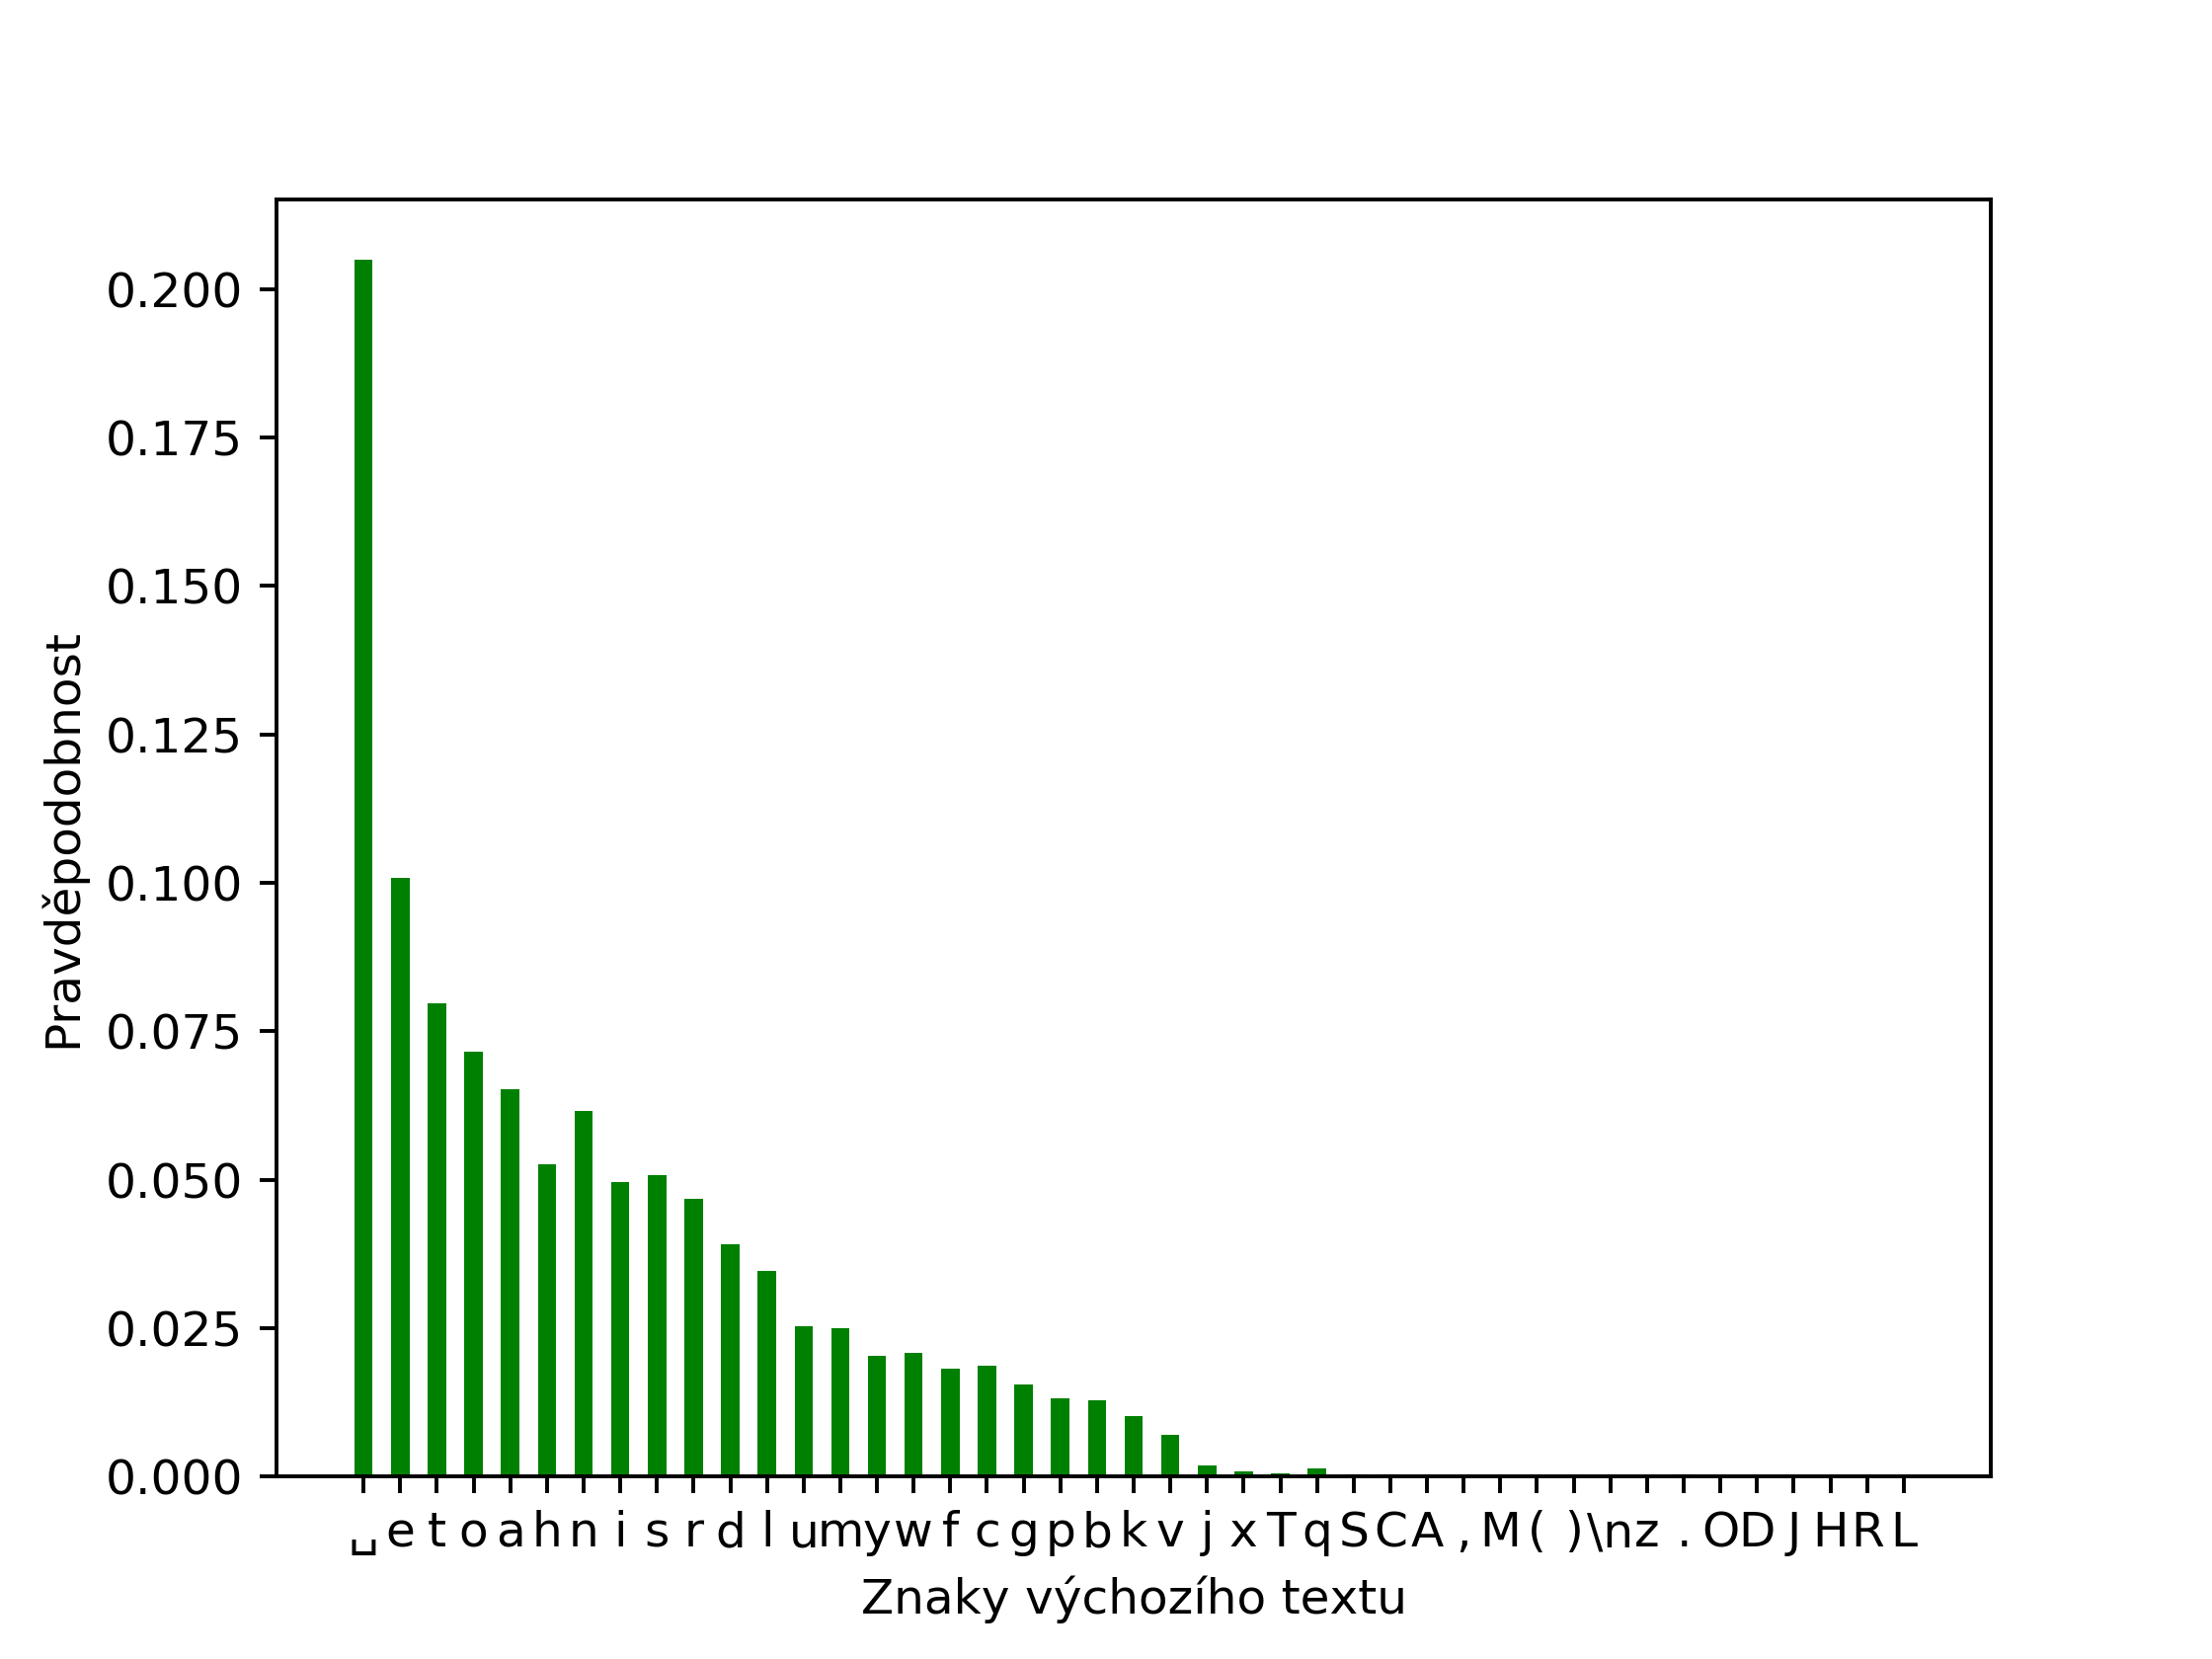
\includegraphics[scale=0.8]{../009_char_prob.png}\centering\caption{Grafické znázornění pravděpodobností znaků textu 009.txt}\label{009_graph}
\end{figure}

\begin{figure}[!htb]
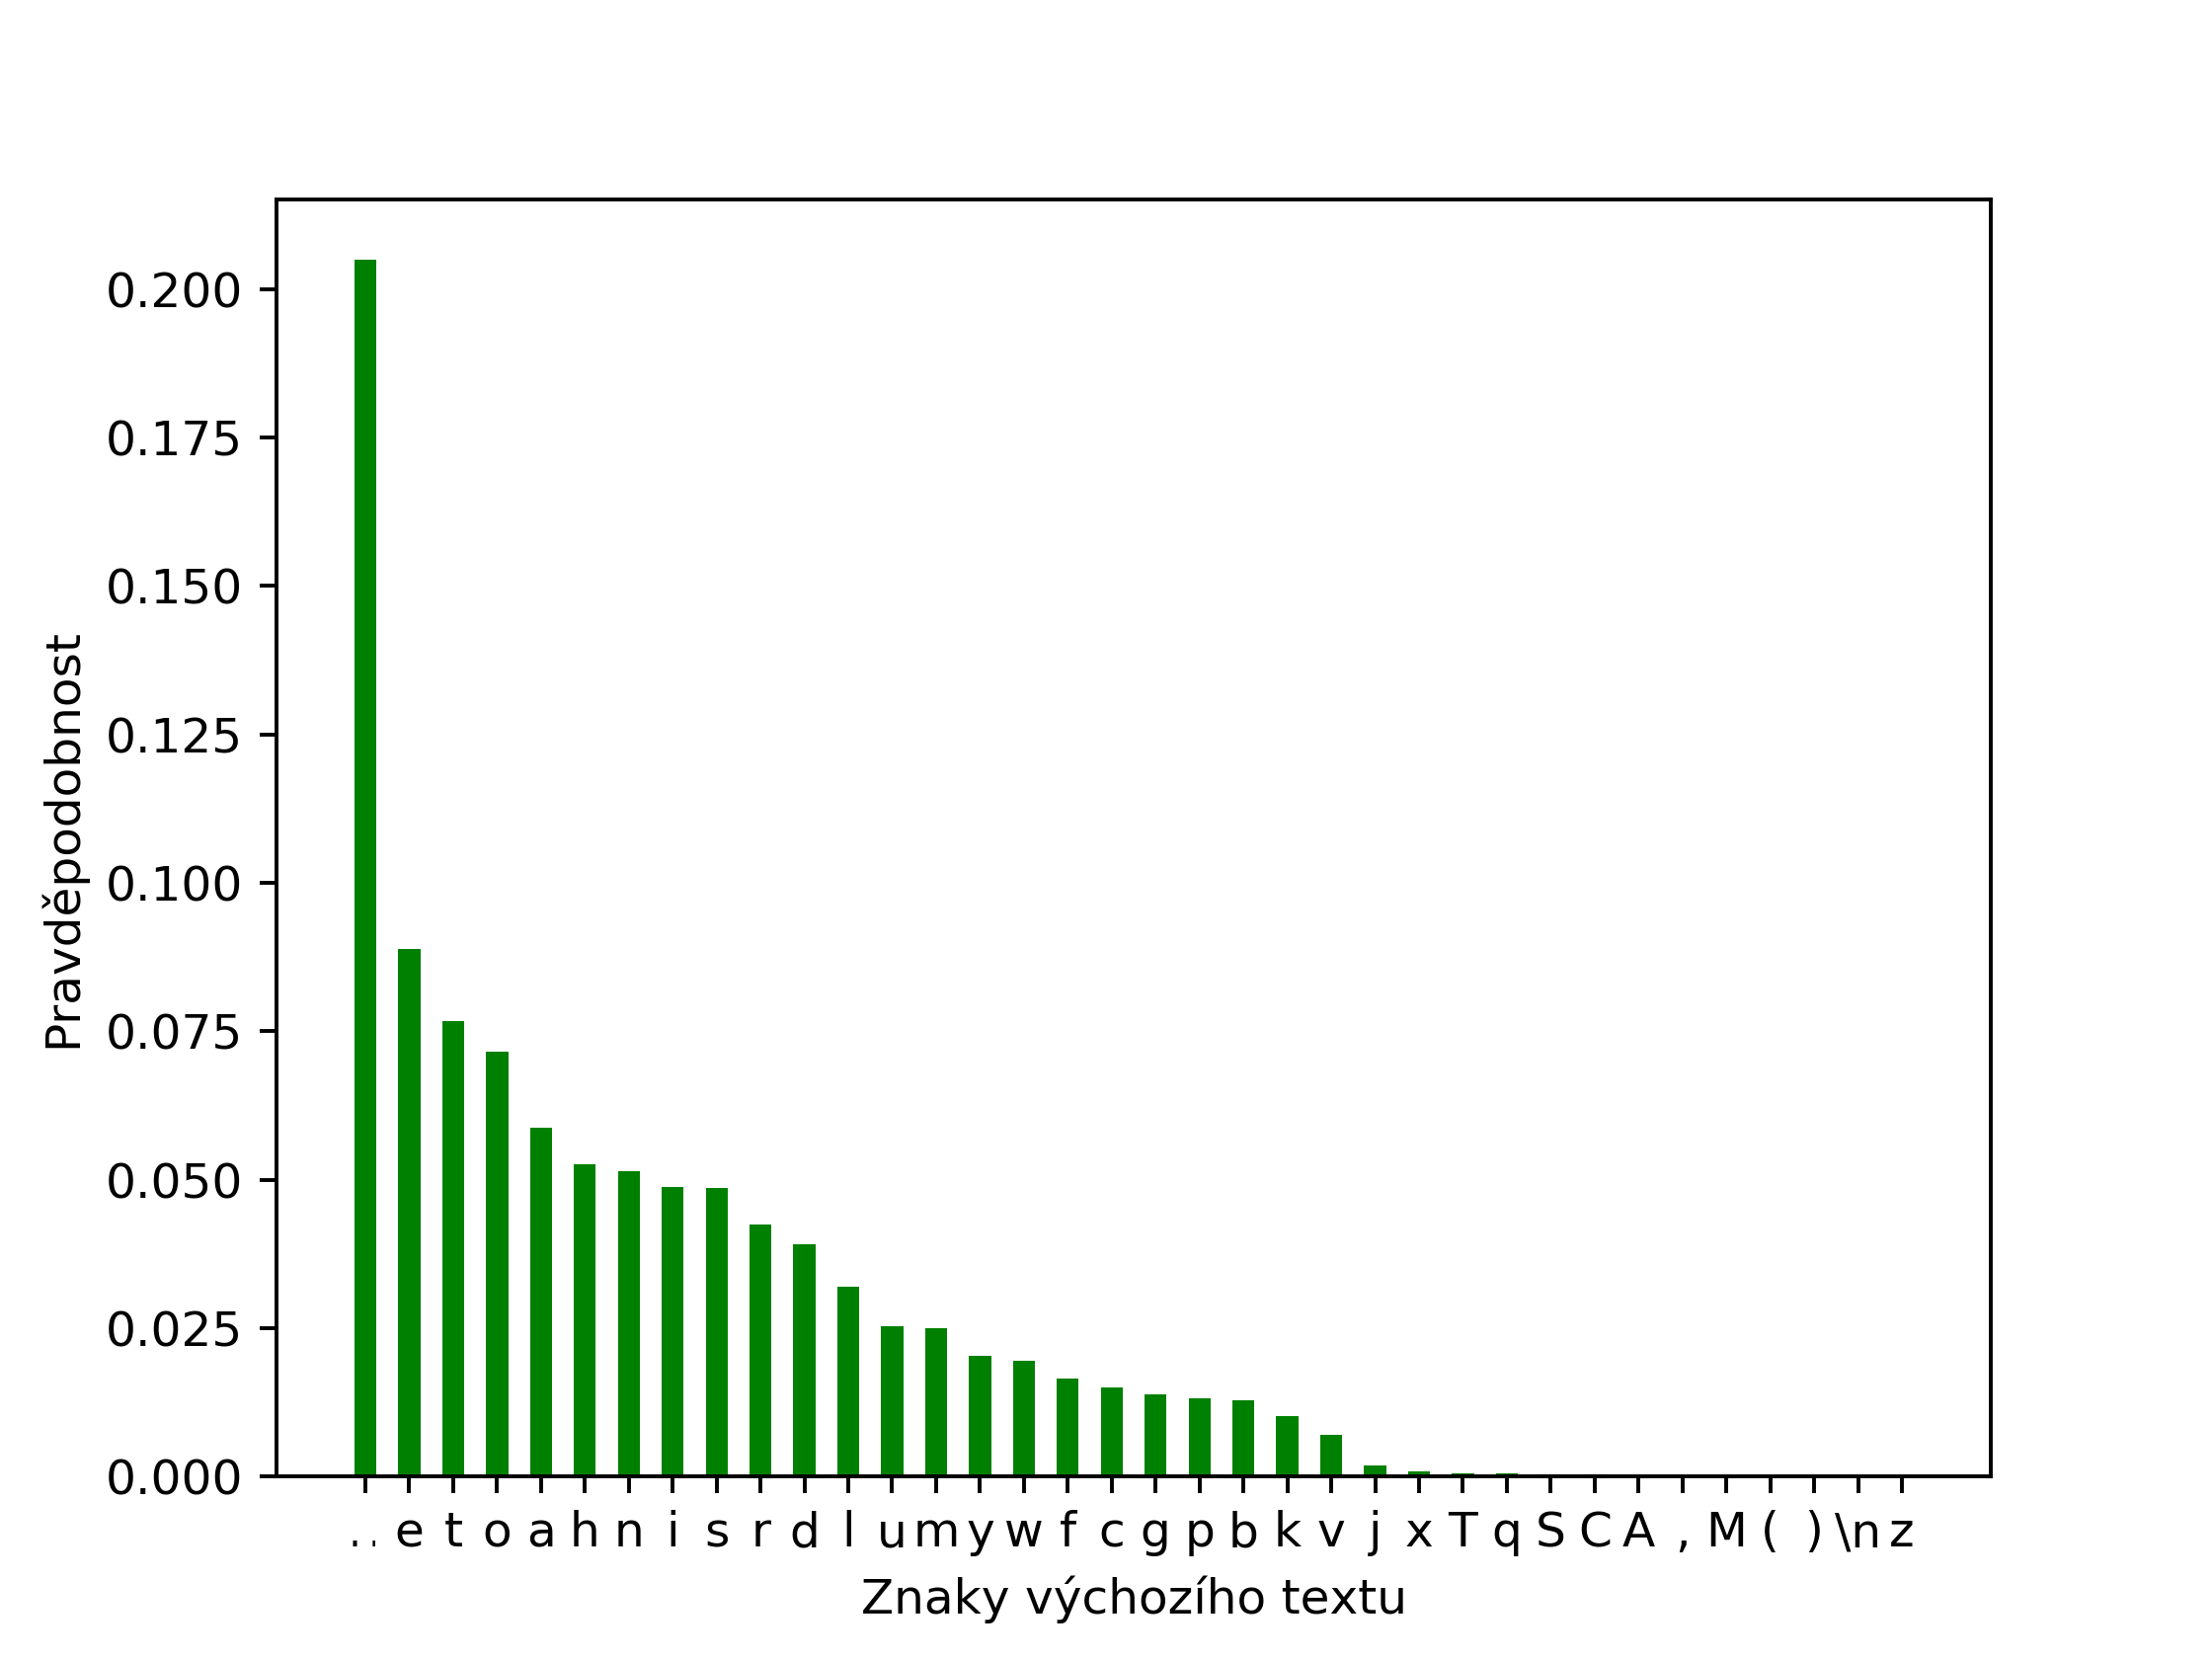
\includegraphics[scale=0.8]{../011_char_prob.png}\centering\caption{Grafické znázornění pravděpodobností znaků textu 011.txt}\label{011_graph}
\end{figure}
		
		
		\subsection{Entropie textů}\label{et}
			Entropie obou textů byla vypočítána na základě zjištěných pravděpodobností následujícím vzorcem. 

			$$ H(X) = -\sum_{x \displaystyle \in X} p(x) log_2 p(x)$$

\begin{table}[!ht]
\centering
\begin{tabular}{ | c | l | } \hline
Text	& Entropie \\ \hline
009.txt & 4.060006550506617 \\ \hline
011.txt & 4.0639057100402844 \\ \hline
\end{tabular}
\caption{Entropie znaků obou textů}
\label{ent_table}
\end{table}
			
			
			
			
		\subsection{Optimální instantní kód}\label{oik}
			Pro nalezení optimálního kódu byl použit algoritmus sestrojení binárního Huffmanova kódu. Implementace tohoto algoritmu je provedena pomocí prioritní fronty a binárního stromu. Fronta je naplněna stavy, které obsahují jednotlivé znaky a je seřazena podle jejich pravděpodobnosti. Dva stavy s nejmenší pravděpodobností jsou vždy spojeny v jeden nový, který je zařazen do binárního stromu. Takto vytvořený stav obsahuje ukazatele na potomky, ze kterých byl sestaven a jejich sečtenou pravděpodobnost. 
			
			Tento postup se opakuje, dokud nezůstane poslední stav ve frontě. Výsledný kód je získán průchodem vzniklým binárním stromem až do listů. Cesta do listu určuje podobu kódového slova znaku, který se v něm nachází.
			
			Takto nalezené optimální kódy pro oba texty jsou zobrazeny v tabulkách \ref{pzhk_009.txt_table} a \ref{pzhk_011.txt_table}.
			
			\begin{table}[!ht]
\centering
\begin{tabular}{ | c | l | r | } \hline
Znak    &       Pravděpodobnost &       Kód     \\ \hline
"\textvisiblespace "    &       0.1898870360408822      &       00      \\ \hline
"e"     &       0.10059171597633136     &       010     \\ \hline
"t"     &       0.08015061861215707     &       1101    \\ \hline
"a"     &       0.0656266810112964      &       1010    \\ \hline
"o"     &       0.06401291016675632     &       1001    \\ \hline
"n"     &       0.06168190783575399     &       1000    \\ \hline
"s"     &       0.05092343553882015     &       0110    \\ \hline
"i"     &       0.05002689618074233     &       11111   \\ \hline
"h"     &       0.04948897256589564     &       11110   \\ \hline
"r"     &       0.046620046620046623    &       11101   \\ \hline
"d"     &       0.036758113681190606    &       11000   \\ \hline
"l"     &       0.0347857270934194      &       10110   \\ \hline
"w"     &       0.021158328850636544    &       111001  \\ \hline
"u"     &       0.019903173749327596    &       111000  \\ \hline
"m"     &       0.019544558006096467    &       110011  \\ \hline
"c"     &       0.018827326519634213    &       110010  \\ \hline
"f"     &       0.01828940290478752     &       101111  \\ \hline
"y"     &       0.017034247803478574    &       101110  \\ \hline
"g"     &       0.015599784830554062    &       011110  \\ \hline
"b"     &       0.011655011655011656    &       011100  \\ \hline
"p"     &       0.011655011655011656    &       011101  \\ \hline
"k"     &       0.006634391249775865    &       0111110 \\ \hline
"v"     &       0.006096467634929173    &       01111111        \\ \hline
"q"     &       0.0014344629729245114   &       011111100       \\ \hline
"j"     &       0.0012551551013089475   &       0111111011      \\ \hline
"x"     &       0.00035861574323112785  &       0111111010      \\ \hline
\end{tabular}
\caption{Pravděpodobnosti znaků a Huffmanův kód sada 009.txt.}
\label{pzhk_009.txt_table}
\end{table}
   		

\begin{table}[!ht]
\centering
\begin{tabular}{ | c | l | r | } \hline
Znak    &       Pravděpodobnost &       Kód     \\ \hline
"\textvisiblespace "    &       0.20561816103217376     &       01      \\ \hline
"e"     &       0.08835538134901193     &       1110    \\ \hline
"t"     &       0.07724971419238935     &       1100    \\ \hline
"o"     &       0.07186019924873428     &       1011    \\ \hline
"a"     &       0.05879470847623714     &       1001    \\ \hline
"h"     &       0.05307855626326964     &       0011    \\ \hline
"n"     &       0.0514453699167075      &       0010    \\ \hline
"i"     &       0.049158909031520495    &       0000    \\ \hline
"s"     &       0.04883227176220807     &       11111   \\ \hline
"r"     &       0.04246284501061571     &       11110   \\ \hline
"d"     &       0.03935979095214764     &       11010   \\ \hline
"l"     &       0.03184713375796178     &       10100   \\ \hline
"u"     &       0.025314388371713212    &       00011   \\ \hline
"m"     &       0.024661113833088357    &       00010   \\ \hline
"y"     &       0.02025151069737057     &       110110  \\ \hline
"w"     &       0.019434917524089497    &       101011  \\ \hline
"f"     &       0.01649518210027764     &       101010  \\ \hline
"c"     &       0.015188633023027927    &       100011  \\ \hline
"g"     &       0.014045402580434428    &       100010  \\ \hline
"p"     &       0.013228809407153356    &       100001  \\ \hline
"b"     &       0.012902172137840928    &       100000  \\ \hline
"k"     &       0.010125755348685286    &       1101110 \\ \hline
"v"     &       0.006859382655560999    &       11011111        \\ \hline
"j"     &       0.0019598236158745713   &       110111101       \\ \hline
"x"     &       0.0008165931732810714   &       1101111001      \\ \hline
"q"     &       0.0004899559039686428   &       11011110001     \\ \hline
"z"     &       0.00016331863465621427  &       11011110000     \\ \hline
\end{tabular}
\caption{Pravděpodobnosti znaků a Huffmanův kód sada 011.txt.}
\label{pzhk_011.txt_table}
\end{table}   		
 
			
   		\subsection{Střední délka kódu}\label{sdk}
			Střední délka optimálního kódu sestaveného pro text 009.txt je pro oba texty vypočítána pomocí následujícího vzorce.
			
			$$ L(C) = \sum_{x \displaystyle \in X} l(x) p(x)$$		
   		
\begin{table}[!ht]
\centering
\begin{tabular}{ | c | l | l | l | } \hline
Text	& Entropie & Délka CC kódu pro 009.txt & Délka CC kódu pro 011.txt \\ \hline
009.txt & 4.060006550506617 & 4.105791644253182 & 4.119956966110813 \\ \hline
011.txt & 4.0639057100402844 & 4.1156295933366   & 4.101420872121509 \\ \hline
\end{tabular}
\caption{Délka Huffmanova kódu sestaveného pro oba texty}
\label{code_table}
\end{table}


   	\section{Závěr}\label{z}
   		Nejpravděpodobnějším znakem obou zkoumaných textů byla mezera. Jako další dva nejvíce pravděpodobné znaky vychází písmena \uv{e} a \uv{t}. To odpovídá standardní frekvenci těchto znaků pro anglický text.
   		
   		Entropie byla pro oba texty téměř shodná, po zaokrouhlení rovna 4,1.
   		
   		Optimální kód byl nalezen pomocí Huffmanova algoritmu pro oba texty. Kódová slova pro nejvíce frekventované znaky jsou dle očekávaní nejkratší. Optimální kód pro druhý text nebylo dle zadání potřeba konstruovat, jeho podobu uvádíme pouze pro porovnání.
   		
   		Pro optimální kód platí dle předpokladů nerovnost:
   		
   		$$ H(X) \leq L(CC) < H(X) + 1 $$
   		
   		
   		

\end{document}